\documentclass{standalone}


\usepackage[europeanresistors,americaninductors]{circuitikz}

\begin{document}
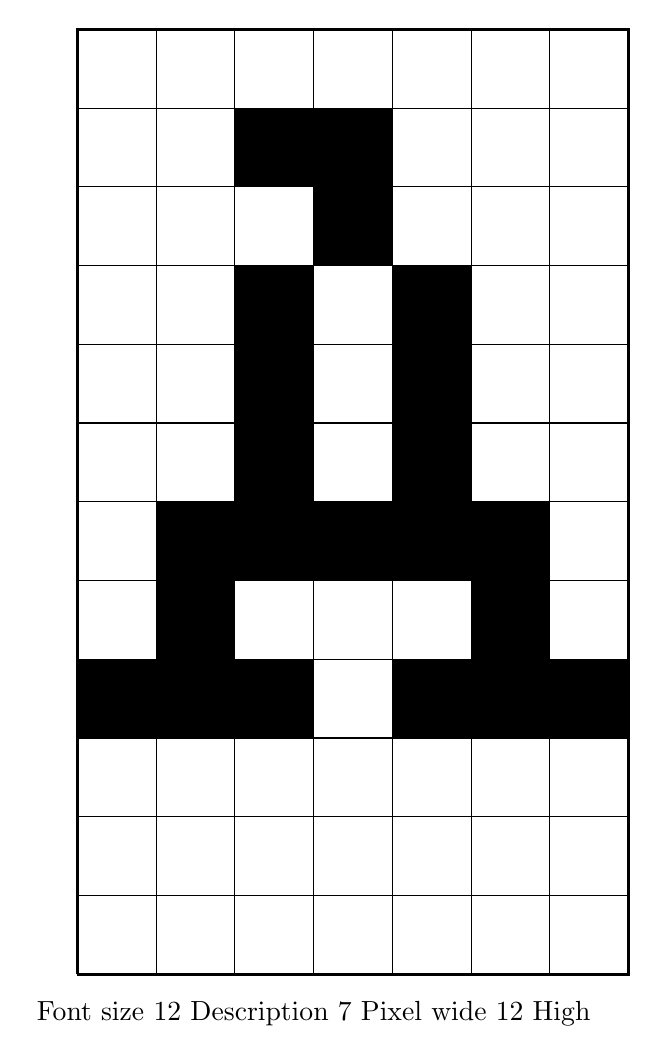
\begin{tikzpicture}

  \begin{scope}
\draw (0, 0) grid (7, 12);
\draw[very thick] (0,0) -- (7,0) -- (7,12) -- (0,12) -- (0,0);
\draw [fill=black] (0,3) rectangle (3,4);
\draw [fill=black] (4,3) rectangle (7,4);
\draw [fill=black] (1,4) rectangle (2,5);
\draw [fill=black] (5,4) rectangle (6,5);
\draw [fill=black] (1,5) rectangle (6,6);
\draw [fill=black] (2,6) rectangle (3,9);
\draw [fill=black] (4,6) rectangle (5,9);
\draw [fill=black] (3,9) rectangle (4,10);
\draw [fill=black] (2,10) rectangle (4,11);




\node[anchor=center] at (3, -0.5) {Font size 12 Description 7 Pixel wide 12 High};
\end{scope}


\end{tikzpicture}
\end{document}
